\documentclass[a4paper,12pt]{article}
\usepackage[top = 2.5cm, bottom = 2.5cm, left = 2.5cm, right = 2.5cm]{geometry}
\usepackage[T1]{fontenc}
\usepackage[utf8]{inputenc}
\usepackage{multirow} 
\usepackage{booktabs} 
\usepackage{graphicx}
\usepackage[spanish]{babel}
\usepackage{setspace}
\setlength{\parindent}{0in}
\usepackage{float}
\usepackage{fancyhdr}
\usepackage{amsmath}
\usepackage{amssymb}
\usepackage{amsthm}
\usepackage[numbers]{natbib}
\newcommand\Mycite[1]{%
	\citeauthor{#1}~[\citeyear{#1}]}
\usepackage{graphicx}
\usepackage{subcaption}
\usepackage{booktabs}
\usepackage{etoolbox}
\usepackage{minibox}
\usepackage{hyperref}
\usepackage{xcolor}
\usepackage[normalem]{ulem}
 \useunder{\uline}{\ul}{}
\usepackage[skins]{tcolorbox}
%---------------------------

\newtcolorbox{cajita}[1][]{
	 #1
}

\newenvironment{sol}
{\renewcommand\qedsymbol{$\square$}\begin{proof}[\textbf{Solución.}]}
	{\end{proof}}

\newenvironment{dem}
{\renewcommand\qedsymbol{$\blacksquare$}\begin{proof}[\textbf{Demostración.}]}
	{\end{proof}}

\newtheorem{problema}{Problema}
\newtheorem{definicion}{Definición}
\newtheorem{ejemplo}{Ejemplo}
\newtheorem{teorema}{Teorema}
\newtheorem{corolario}{Corolario}[teorema]
\newtheorem{lema}[teorema]{Lema}
\newtheorem{prop}{Proposición}
\newtheorem*{nota}{\textbf{NOTA}}
\renewcommand\qedsymbol{$\blacksquare$}
\usepackage{svg}
\usepackage{tikz}
\usepackage[framemethod=default]{mdframed}
\global\mdfdefinestyle{exampledefault}{%
linecolor=lightgray,linewidth=1pt,%
leftmargin=1cm,rightmargin=1cm,
}




\newenvironment{noter}[1]{%
\mdfsetup{%
frametitle={\tikz\node[fill=white,rectangle,inner sep=0pt,outer sep=0pt]{#1};},
frametitleaboveskip=-0.5\ht\strutbox,
frametitlealignment=\raggedright
}%
\begin{mdframed}[style=exampledefault]
}{\end{mdframed}}
\newcommand{\linea}{\noindent\rule{\textwidth}{3pt}}
\newcommand{\linita}{\noindent\rule{\textwidth}{1pt}}

\AtBeginEnvironment{align}{\setcounter{equation}{0}}
\pagestyle{fancy}

\fancyhf{}









%----------------------------------------------------------
\lhead{\footnotesize Geometría Moderna}
\rhead{\footnotesize  Rudik Roberto Rompich}
\cfoot{\footnotesize \thepage}


%--------------------------

\begin{document}
 \thispagestyle{empty} 
    \begin{tabular}{p{15.5cm}}
    \begin{tabbing}
    \textbf{Universidad del Valle de Guatemala} \\
    Departamento de Matemática\\
    Licenciatura en Matemática Aplicada\\\\
   \textbf{Estudiante:} Rudik Roberto Rompich\\
   \textbf{Correo:}  \href{mailto:rom19857@uvg.edu.gt}{rom19857@uvg.edu.gt}\\
   \textbf{Carné:} 19857
    \end{tabbing}
    \begin{center}
        MM2031 - Geometría Moderna - Catedrático: María Eugenia Contreras Pinillos\\
        \today
    \end{center}\\
    \hline
    \\
    \end{tabular} 
    \vspace*{0.3cm} 
    \begin{center} 
    {\Large \bf  HT 1
} 
        \vspace{2mm}
    \end{center}
    \vspace{0.4cm}
%--------------------------

\begin{problema}
	Tangentes a las circunferencias en $A^{\prime}$ y $B$ forman ángulos iguales con la línea $A^{\prime} B $. Si estas tangentes se intersecan en $E$ el triángulo $E A^{\prime} B$ es isósceles.
	\begin{figure}[H]
		\centering
		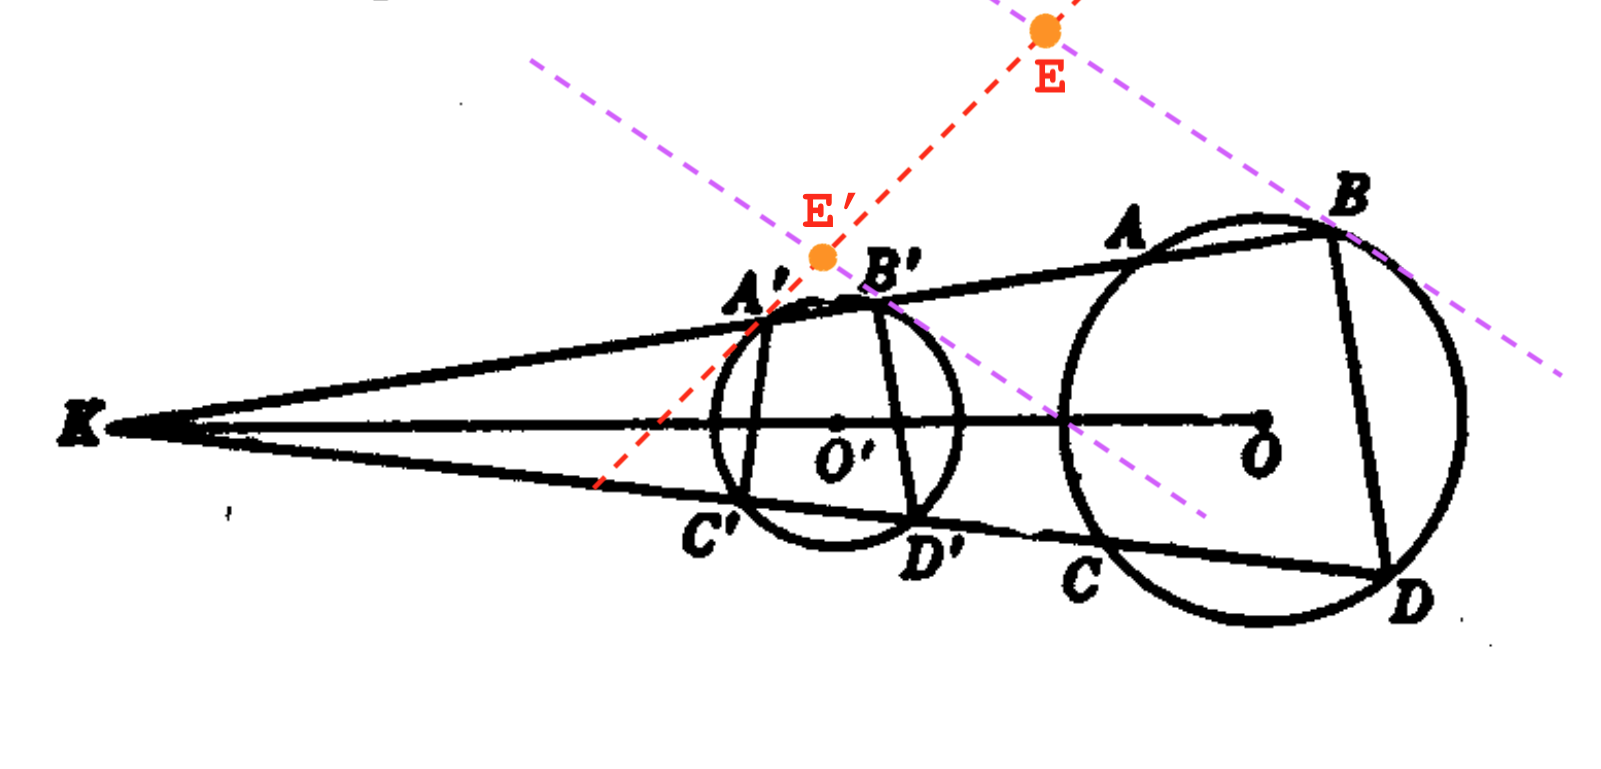
\includegraphics[scale=0.2]{Images/1}
	\end{figure}
\end{problema}
\begin{proof}
	Nótese que por hipótesis $A',A,B,B',C,C'$ y $D,D'$ son homólogos. $\implies$ Como las circunferencias son homotéticas, entonces la tangente que pasa por $BE$ es paralela a la tangente que pasa por  $B'E'$ tal que $BE'\parallel B'E$. $\implies$ Por el teorema de paralelas y transversas $\angle A'B'E' = \angle A'B'E$. $\implies$ Por la definición de tangentes a circunferencias $\angle E'A'B' = \angle A'B'E'$. $\implies \triangle E'A'B'$ es isósceles. $\implies$ Por congruencia de los ángulos y teorema de similaridad para triángulos $\angle EA'B = \angle A'BE$. Por lo tanto, $\triangle EA'B$ es isósceles.
\end{proof}


\begin{problema}
	 La circunferencia de similitud de dos circunferencias no concéntricas es el lugar geométrico de los puntos (1) tales que las razones de sus distancias a los centros de las circunferencias son iguales a las razones entre los radios; $y$ (2) desde los cuales las dos circunferencias subtienden ángulos iguales.
	 \begin{figure}[H]
	 	\centering
	 	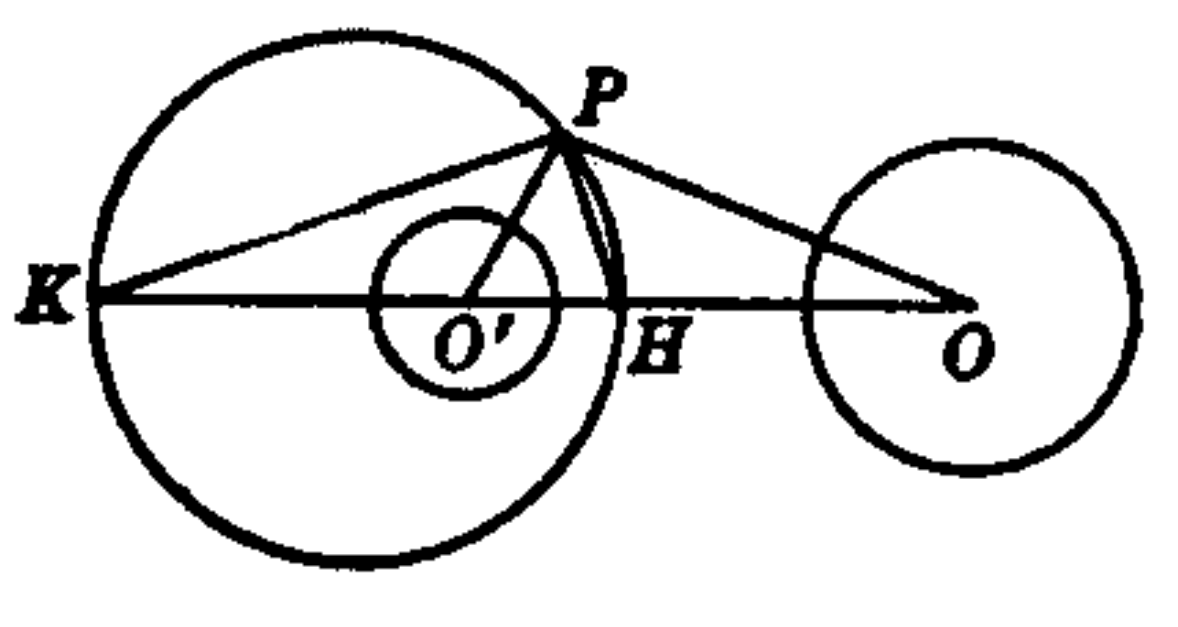
\includegraphics[scale=0.2]{Images/2}
	 \end{figure}
\end{problema}
\begin{proof}
	A probar: 
	\begin{enumerate}
		\item $P\in$ circunferencia de similitud $\implies PO/PO'=r/r'$. Supóngase que tenemos un punto $O''$ en el segmento de los centros, tal que el segmento $PH$ es la bisectriz de $\angle O''PO'$. $\implies$ Por el teorema de Thales, $PH \perp PK$ bisectan los $\angle$ interiores y exteriores en $P$ de $\triangle O''PO'$. $\implies$ 
		$$\frac{O''H}{HO'}= -\frac{O''K}{KO'}\quad \text{y} \quad \frac{OH}{HO'}=-\frac{OK}{KO'}\implies \frac{H}{O''}\frac{O''}{K}=\frac{HO}{OK}\implies O''=O.$$
		Por lo tanto, $$\frac{PO}{PO'}=\frac{r}{r'}.$$
		\item $PO/PO'=r/r\implies P\in$ circunferencia de similitud.  Por el teorema de la bisectriz,  $PH$ es la bisectriz del $\angle$ interior en $P$ de $\triangle OPO'$. Por otra parte, por el teorema de la bisectriz $PK$ es la bisectriz del $\angle$ exterior en $P$ de $\triangle OPO'$. Por lo tanto, $PH\perp  PK$ y $P\in $ circunferencia de similitud. 
	\end{enumerate}
\end{proof}

%---------------------------
\bibliographystyle{apa}
\bibliography{referencias.bib}

\end{document}